\chapter{Reducing the computational cost}
\label{ch:reducing}

As emphasized in section \ref{sec:general-presentation}, neighbourhood component analysis (NCA) is a computationally expensive method. The evaluation of its objective function is quadratic in the size of the data set. Given that the optimization is done iteratively, NCA becomes prohibitively slow when applied on large data sets. There is only little previous work that uses NCA for large scaled applications. One example is \citet{singh2010}, who parallelizes the computations across multiple computers and adopts various heuristics to prune terms of the objective function and the gradient.

This chapter aims to continue the existing work and to present a series of methods that can improve NCA's speed. Most of these ideas are new in the context of NCA. We start with simple approaches like sub-sampling (section~\ref{sec:sub-sampling}) and mini-batch methods (sections~\ref{sec:mini-batches} and~\ref{sec:stochastic-learning}). For further speed-ups, we proceed with more sophisticated ideas (starting from section~\ref{sec:approximate}). 
%They are also quite versatile. Each method proposes a new objective function and can be regarded as an independent model on its own.

% \begin{itemize}
% 	\item As mentioned in section , evaluating the objective function needs
% computing all the pairwise distances between the points. Also, the evaluating
% the gradient is expensive. This is done in $\mathcal{O}(N^2D^2)$ flops. So it is
% not trivial to successfully use NCA on large data sets.
% 	\item  Most of the methods rely on the fact that
% the learnt metric is low ranked.
% 	\item Every method presented can be regarded as an alteration of the original
% objective function. We basically change our objective function such that the new
% objective will have a reduced cost.
% \end{itemize}

\section{Sub-sampling}
\label{sec:sub-sampling}

Sub-sampling is the simplest idea that can help speeding up the computations.
For the training procedure we use a randomly selected sub-set $\mathcal{D}_n$ of
the original data set $\mathcal{D}$:
 \[
 	\mathcal{D}_n = \{ \xB_{i_1},\cdots,\xB_{i_n} \} \subseteq \mathcal{D}.
 \]
 If $n$ is the size of the sub-set then the cost of the gradient, equation~\eqref{eq:nca-grad-alt}, is reduced to
$\mathcal{O}(dDn^2)$. After the projection matrix $\AB$ is learnt, we apply it to the whole data set $\{\xB_i\}_{i=1}^N$. Then all the new data points $\{\AB\xB_i\}_{i=1}^N$ are used for
classification. The cost of the classification is $\mathcal{O}(dN)$ which is linear in the total number of points $N$.

While easy to implement, this method discards a lot of the information available.
Also it is affected by the fact the sub-sampled data has a thinner density
than the real data. The distances between the randomly selected points are larger than they are in the full data set. This causes the scale of the projection matrix $\AB$ not to be large enough. In figure \ref{fig:sub-sampling} we illustrate that a seemingly perfect linear transformation of the sub-sampled data set does not correspond to a good transformation of the entire data set.

\begin{figure}
  \centering
  \subfigure[Learnt projection $\AB$ on the sub-sampled data set
$\mathcal{D}_n$.]{\label{fig:sub-sampling-1}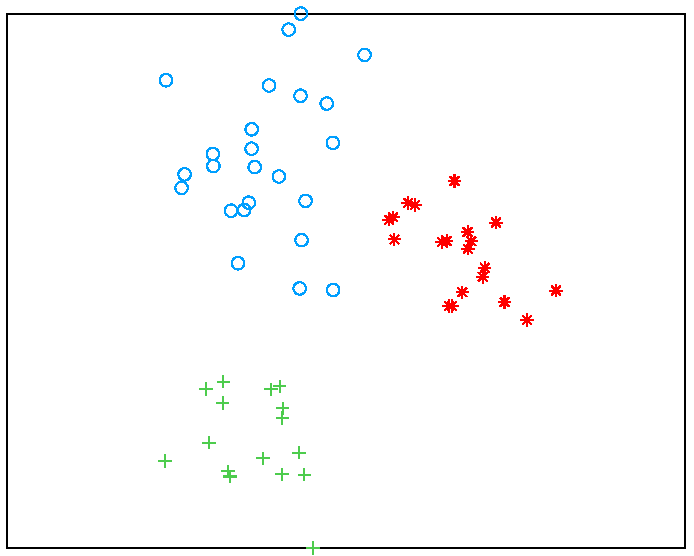
\includegraphics[width=0.48\textwidth]{images/sub-sample-1}}
\subfigure[The projection $\AB$ applied to the whole data set
$\mathcal{D}$.]{\label{fig:sub-sampling-2}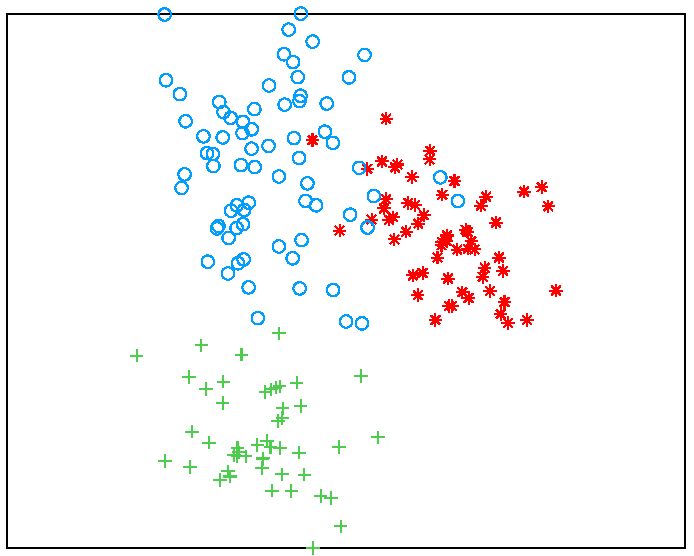
\includegraphics[width=0.48\textwidth]{images/sub-sample-2}}
  \caption[Associated problems with sub-sampling method]{Result of sub-sampling method on \texttt{wine}. One
third of the original data set were used for training, i.e., $n = N/3$. We note
that the points that belong to the sub-set~$\mathcal{D}_n$ are perfectly
separated. But after applying the metric to the whole data, misclassification errors appear. The effects are more acute if we use smaller
sub-sets.}
  \label{fig:sub-sampling}
\end{figure}

\section{Mini-batches}
\label{sec:mini-batches}

The next obvious idea is to use sub-sets of data in an iterative manner, similarly to the
stochastic gradient descent method: split the data into mini-batches and train
on them successively. Again the cost for one evaluation of the gradient will be
$\mathcal{O}(dDn^2)$ if the mini-batch consists of $n$ points. 

A possible way of using mini-batches for learning an NCA projection is summarized by algorithm \ref{alg:mini-batches}. We remind that important characteristics of the algorithm (such as convergence, the learning rate or initialization) were discussed in sections~\ref{subsec:optimization} and~\ref{subsec:initialization}.

\begin{algorithm} 
	\caption{NCA learning algorithm using mini-batches (NCA MB)} 
	\label{alg:mini-batches}  
	\begin{algorithmic} [1]                 % enter the algorithmic environment
		\REQUIRE Data set $\mathcal{D}=\{\xB_1,\cdots,\xB_N\}$ and initial linear
transformation $\AB$.
		\REPEAT
			\STATE Project each data point using $\AB$: 
$\mathcal{D}_\AB=\{\AB\xB_1,\cdots,\AB\xB_N\}$.
			\STATE Use either algorithm \ref{alg:fpc} or \ref{alg:rpc} on
$\mathcal{D}_\AB$ to split $\mathcal{D}$  into $K$ mini-batches
$\mathcal{M}_1,\cdots,\mathcal{M}_K$.
			\FORALL {$\mathcal{M}_i$}
				\STATE {Update parameter: $\AB\leftarrow \AB + \eta\frac{\partial
f(\AB,\mathcal{M}_i)}{\partial\AB}$.}
				\STATE {Update learning rate $\eta$.}
			\ENDFOR
		\UNTIL {convergence.}
	\end{algorithmic}
\end{algorithm}

We considered two different choices for splitting the data-set:
\begin{description}
	\item[Random selection.] In this case the points are assigned randomly to each
mini-batch. After one pass through the whole data set, we repeat the random
allocation procedure. As in section \ref{sec:sub-sampling}, this suffers from the
thin distribution problem. In order to alleviate this problem and achieve convergence,
we should use large-sized mini-batches (as in the NCA
implementation of \citealp{maaten-online}). The algorithm is similar to algorithm \ref{alg:mini-batches},
but lines 2 and 3 will be replaced with a simple random selection.
	
	\item[Clustering.] Constructing mini-batches by clustering ensures that the
point density in each mini-batch is conserved. In order to maintain a low
computational cost, we consider cheap clustering methods, e.g.,
farthest point clustering (FPC; \citealp{gonzalez1985}) and recursive projection
clustering (RPC; \citealp{chalupka2011}).  
	
	FPC gradually selects cluster centres until it reaches the desired number of
clusters $K$. The point which is the farthest away from all the current centres
is selected as the new centre. The precise procedure is given by algorithm \ref{alg:fpc}.
	
	\begin{algorithm} 
		\caption{Farthest point clustering (FPC; \citealp{gonzalez1985})} 
		\label{alg:fpc}  
		\begin{algorithmic}[1]                    % enter the algorithmic environment
			\REQUIRE Data set $\mathcal{D}=\{\xB_1,\cdots,\xB_N\}$ and $K$ number of
clusters.
			\STATE Randomly pick a point that will be the first centre $\cB_1$.
			\STATE Allocate all the points in the first cluster $\mathcal{M}_1 \leftarrow
\mathcal{D}$.
			\FOR {$i=1$ to $K$}
				\STATE Select the $i$-th cluster centre $\cB_i$ as the point that is
farthest away from any cluster centre $\cB_1,\cdots,\cB_{i-1}$.
				\STATE Move to the cluster $\mathcal{M}_i$ those points that are closer to
its centre than to any other cluster centre: $\mathcal{M}_i = \left\{ \xB \in
\mathcal{D} \;| \; d(\xB;\cB_i) < d(\xB;\cB_j), \forall j \neq i \right\}$
			\ENDFOR
		\end{algorithmic}
	\end{algorithm}
	
	The computational cost of this method is $\mathcal{O}(NK)$. However, we do not
have any control on the number of points in each cluster, so we might end up
with very unbalanced clusters. A very uneven split has a couple of obvious
drawbacks: too large mini-batches will maintain high cost, while on too small
clusters there is not too much to learn.
	
	An alternative is RPC which was especially designed to mitigate this problem.
It constructs the clusters similarly to how the $k$-d trees are build, (subsection~\ref{subsec:k-d-trees}). But instead of splitting the data set across axis aligned
directions it chooses the splitting directions randomly (algorithm~\ref{alg:rpc}). Because RPC uses the median value it will result in similar
sized clusters and we can easily control the dimension of each cluster. 
% The complexity of this algorithm is $\mathcal{O}()$.
	
	\begin{algorithm} 
		\caption{Recursive projection clustering (RPC; \citealp{chalupka2011})} 
		\label{alg:rpc}  
		\begin{algorithmic}[1]                    % enter the algorithmic environment
			\REQUIRE Data set $\mathcal{D}=\{\xB_1,\cdots,\xB_N\}$ and $n$ size of
clusters.
			\IF {$N < n$}
				\STATE New cluster: $i\leftarrow i+1$.
				\RETURN current points as a cluster: $\mathcal{M}_i \leftarrow \mathcal{D}$.
			\ELSE
				\STATE {Randomly select two points $\xB_j$ and $\xB_k$ from $\mathcal{D}$.}
				\STATE {Project all data points onto the line defined by $\xB_j$ and
$\xB_k$.}
				\STATE {Select the median value $\tilde{\xB}$ from the projected points.}
				\STATE {Recurs on the data points above and below $\tilde{\xB}$:
$\text{RPC}(\mathcal{D}_{>\tilde{\xB}})$ and
$\text{RPC}(\mathcal{D}_{\le\tilde{\xB}})$.}
%							$\mathcal{D}_{>\tilde{\xB}}=\{\xB\in\mathcal{D}|\xB>\tilde{\xB}\}$
			\ENDIF
		\end{algorithmic}
	\end{algorithm}
\end{description}

	In algorithm~\ref{alg:mini-batches}, we are re-clustering in the transformed space after one sweep through
the whole data set. There are other alternatives. For example, we could
cluster in the original space, either once or periodically. The proposed variant works well in the case of a low-rank projection matrix~$\AB$: we obtain better clusters using RPC on low dimensional data sets than on high dimensional data sets.
%First it is cheaper, but the clusters resulted in low dimensions by using RPC are closer to the real clusters then applying the same method in a high dimensional space. 

%\begin{center}
%	\begin{table}
%		\centering
%		\begin{tabular}{l}
%			\toprule
%			Training algorithm using mini-batches\\
%			\midrule
%			\textbf{Do}\\
%			Split data $\mathcal{D}$ into mini-batches:
%$\mathcal{M}_1,\cdots,\mathcal{M}_m$,\\
%			such that $\mathcal{M}_1\cup\cdots\cup\mathcal{M}_m=\mathcal{D}$\\
%			\textbf{For each} mini-batch $\mathcal{M}_i$\\
%			$\AB\leftarrow \AB - \eta\frac{\partial
%f(\AB,\mathcal{M}_i)}{\partial\AB}$\\
%			\textbf{End for}\\
%			\textbf{Until} we reach convergence\\
%			\bottomrule
%		\end{tabular}
%		\caption{Algorithm for training with mini-batches. The learning is done using
%gradeint ascent.}
%	\end{table}
%\end{center}


\section{Stochastic learning}
\label{sec:stochastic-learning}

The following technique is theoretically justified by stochastic approximation arguments. The main idea is to get an unbiased estimator of the gradient by
looking only at a few points and how they relate to the \textit{entire} data set. More precisely, at each iteration we randomly select $n$ data points and find their stochastic nearest neighbours assignments using all the data. We maximize the probability of these $n$ points belonging to the true class:
\begin{align}
 	f_\text{NCA-SL}(\AB) &= \sum_{l=1}^n p_{i_l},
\end{align}
where $i_1,\cdots,i_n$ denote the indices of the randomly selected points and $p_i$ is the average probability of the point $i$ of getting correctly classified:
\begin{align}
 p_i &= \sum_{\substack{j=1\\j\in c_i}}^Np_{ij}.
\end{align}

The gradient of the new objective function is given by:
\begin{align}
	\frac{\hat{\partial f}}{\partial \AB}&=\frac{\partial f_\text{NCA-SL}}{\partial \AB} = \sum_{l=1}^{n} \frac{\partial
p_{i_l}}{\partial \AB}\\
	&=2\sum_{l=1}^{n}\left(p_{i_l}\sum_{k=1}^Np_{{i_l}k}(\AB\xB_{{i_l}k})\xB_{{i_l}k}^{\textrm{T}} -
	\sum_{j\in c_{i_l}}p_{{i_l}j}(\AB\xB_{{i_l}j})\xB_{{i_l}j}^{\textrm{T}} \right).
	\label{eq:snca-grad}
\end{align}

The evaluation of the objective function and its gradient scales with $nN$. Algorithm \ref{alg:nca-sl} presents a stochastic learning procedure for NCA. As before, we refer the reader to the previous subsections~\ref{subsec:optimization} and~\ref{subsec:initialization} for advice regarding the convergence and update of the learning rate.

	\begin{algorithm} 
		\caption{Stochastic learning for NCA (NCA SL)} 
		\label{alg:nca-sl}  
		\begin{algorithmic}[1]                    
			\REQUIRE Data set $\mathcal{D}=\{\xB_1,\cdots,\xB_N\}$, $n$ number of points
to consider for the gradient estimation, $\AB$ initial linear transformation.
			\REPEAT
				\STATE Split data $\mathcal{D}$ into groups $\mathcal{M}_i$ of size $n$.\
				\FORALL {$\mathcal{M}_i$}
					\STATE {Update parameter using gradient given by equation
\ref{eq:snca-grad}:\\ $\AB\leftarrow \AB + \eta\frac{\partial
f_\text{NCA-SL}(\AB,\mathcal{M}_i)}{\partial\AB}$.}
					\STATE {Update learning rate $\eta$.}
				\ENDFOR
			\UNTIL {convergence.}
		\end{algorithmic}
	\end{algorithm}

It might be useful to contrast the NCA SL algorithm with the simple NCA. In the classical NCA learning setting, we update our parameter~$\AB$
after we have considered each point $i$ in the data set and how it relates to the rest of the training set. In the stochastic
learning procedure, we update $\AB$ more frequently by considering only $n$
randomly selected points and how they relate to the whole training set. 
%This allows us to have significantly modified the parameter after one sweep through the training data. 
The use of the stochastic gradient is motivated by the fact that at the initial stages we are far from the optimum solution. If we follow a direction that makes an angle smaller than $\pi/2$ with the true gradient, we get closer to the maximum of the function. Estimated gradients often represent a cheap and practical way of optimizing the parameters.

NCA SL also differs from the mini-batcs method because for the mini-batch method the contributions $p_i$ are calculated only between the $n$ points that belong to the mini-batch.
%As in the previous case, we still need to compute the soft assignments $\{p_i\}_{i=1}^n$ using \textit{all} the $N$ points. To stress this further, this solution differs from the mini-batch approach. 

This stochastic learning method method comes with an additional facility. It can be used for on-line learning. Given a
new point $\xB_{N+1}$ we update $\AB$ using the derivative $\frac{\partial
p_{N+1}}{\partial \AB}$.

\section*{Interlude}

The algorithms we presented are characterized by data sub-sampling. These are easy to apply once we decide on the converge conditions and the learning rate update.

In the following sections we describe variants of algorithms that use approximations. When computing $p_i$ we can ignore some of the individual point contributions $p_{ij}$. While useful on their own, this family of algorithms can achieve better accelerations when combined with the previous methods. 

In section~\ref{sec:approximate} we use $k$-d trees to select the significant stochastic assignments $p_{ij}$ that are significant. To clearly present this method, we need to introduce the $k$-d tree data structure (subsection~\ref{subsec:k-d-trees}) and how it is used for fast kernel density estimation (subsection~\ref{subsec:approx-kde}). Subsection~\ref{subsec:approx-KDE-for-NCA} offers details of adapting existing algorithms specifically for NCA. In section~\ref{sec:exact-computations}, we change the NCA model into a compact support version of NCA, such that only the points within a certain radius from the query point are considered, while the rest are given $0$ weight. Lastly, we present a more robust version of the compact support NCA that avoids possible numerical problems (subsection \ref{sec:nca-cs-back}).

\section{Approximate computations}
\label{sec:approximate}

A straightforward way of speeding up the computations was previously mentioned
in the original paper \citep{goldberger2004} and in some NCA related work
\citep{weinberger2007, singh2010}. The observations involve pruning small terms in
the original objective function. We then use an approximated objective function
and its corresponding gradient for the optimization process.

\begin{figure}
	\centering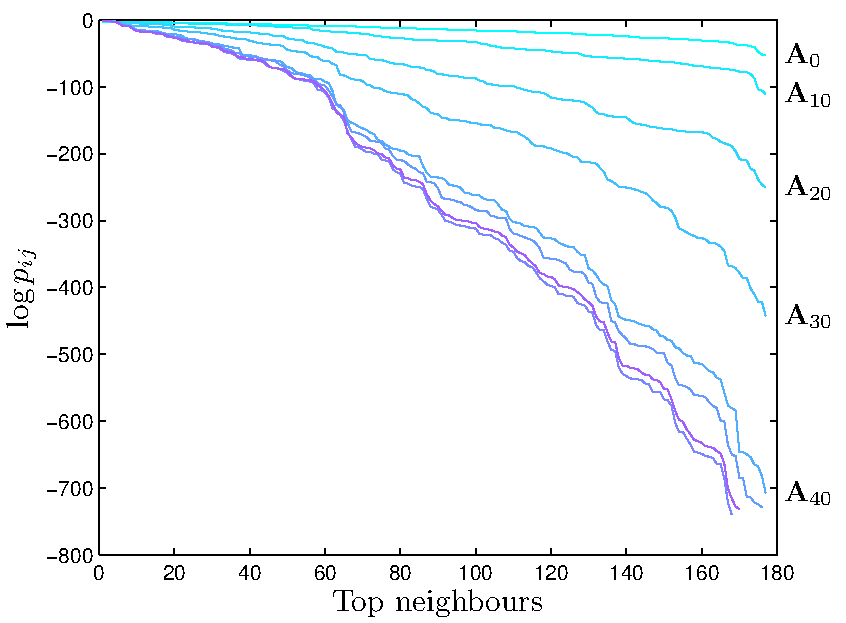
\includegraphics[width=0.7\textwidth]{images/contributions}
	\caption[Evolution of the stochastic assignments $p_{ij}$ during training]{Evolution of the stochastic assignments $p_{ij}$ during training for a given point~$i$. The $y$-axis specifies the contributions $p_{ij}$ on a logarithmic scale. On x-axis we sorted the neighbours in descending order of their contributions. Each curve is associated to a certain linear projection~$\AB_t$, where $t$ denotes the iteration number from the optimization algorithm.}
	\label{fig:contributions}
\end{figure}

The motivation lies in the fact that the contributions $p_{ij}$ decay very
quickly with distance:
 \[
 	p_{ij} \propto \exp\{-d(\AB\xB_i;\AB\xB_j)^2\}.
 \] 
 
The evolution of the contributions during the training period is depicted in
figure \ref{fig:contributions}. We notice that maybe in the first 5-10 iterations the contributions of more than 50 neighbours are significant; after we get out of this regime we can discard a large part of the neighbours and preserve the
accuracy of our estimations. 

\citet{weinberger2007} choose to use only the top $m = 1000$ neighbours for
each point $\xB_i$. Also they disregard those points that are farther away than
$d_{\max}=34$ units from the query point: $p_{ij} = 0, \forall \xB_j$ such that
$d(\AB\xB_i;\AB\xB_j)>d_{\max}$. While useful in practical situations, these
suggestions lack a principled description: how can we optimally choose $m$
and $d_{\max}$ in a general setting? We would also like to be able to estimate
the error introduced by the approximations.

We correct those drawbacks by making use of the KDE formulation of NCA (see
section \ref{sec:cc-kde}) and adapting existing ideas for fast KDE
\citep{deng1995,gray2003} to our particular application. We will use a class of
accelerated methods that are based on data partitioning structures
(e.g., $k$-d trees, ball trees). As we shall see shortly, these provide
us with means to quickly find only the neighbours $\xB_j$ that give significant
values $p_{ij}$ for any query point $\xB_i$. 
%Hence, we will be able to compute an approximated value of the true
%class-conditional probability $p(\xB_i|c) = \sum_{j\in c}
%k(\xB_i|\xB_j),\forall i,c.$
%
%A question still remains: given a point $\xB_i$ how can we \textit{quickly} ?
%It is clear that only the nearby points will contribute to $p_i$, while the
%points that are further away can be ignored. A framework that provides us with
%means of doing this is the $k$-d tree.

\subsection{$k$-d trees}
\label{subsec:k-d-trees}

The $k$ dimensional tree structure ($k$-d tree; \citealp{bentley1975}) organises
the data in a binary tree using axis-aligned splitting planes. The $k$-d tree
places points that live nearby in the 
original geometrical space close in the tree. This makes such structures efficient mechanisms for
nearest neighbour searches \citep{friedman1977} or range searches
\citep{moore1991}.

There are different flavours of $k$-d trees. We choose for our application a
variant of $k$-d tree that uses bounding boxes to describe the position of the
points. Intuitively, we can imagine each node of the tree as a bounding
hyper-rectangle in the $D$ dimensional space of our data. The root node will
represent the whole data set and it can be viewed as a hyper-rectangle that
contains all the data points, see figure \ref{fig:kdtree-1}. In the two-dimensional example presented, the points are enclosed by rectangles. Figures \ref{fig:kdtree-1} to \ref{fig:kdtree-4} show the existing bounding boxes at different levels of the binary tree. To understand how these are obtained, we discuss the $k$-d tree construction.

\begin{figure}
  \centering
  \subfigure[Root
node]{\label{fig:kdtree-1}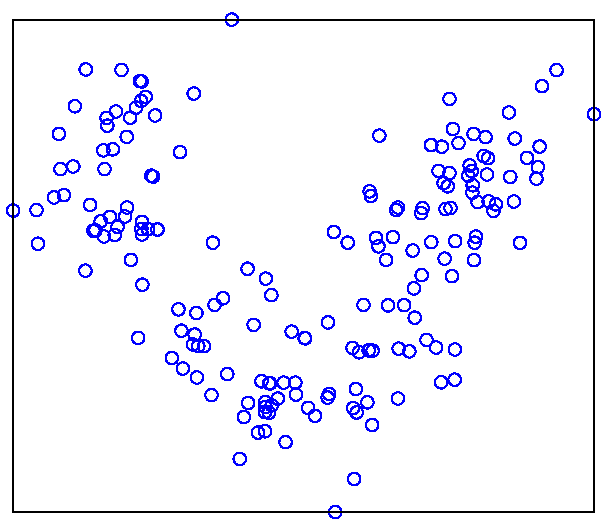
\includegraphics[width=0.45\textwidth]{images/kdtree-1}}
\subfigure[First
level]{\label{fig:kdtree-2}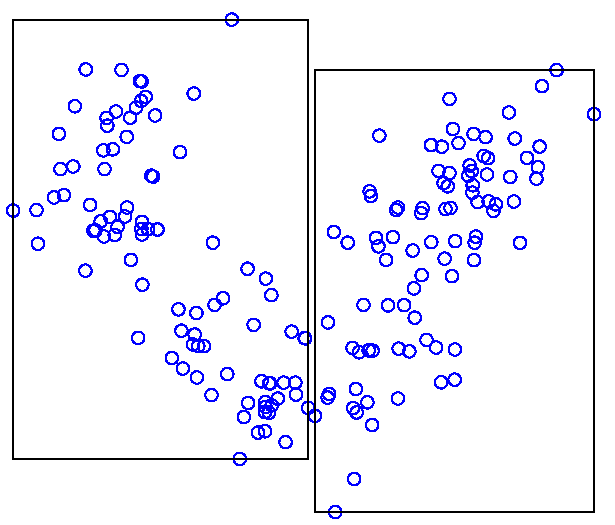
\includegraphics[width=0.45\textwidth]{images/kdtree-2}}
\\
  \subfigure[Second
level]{\label{fig:kdtree-3}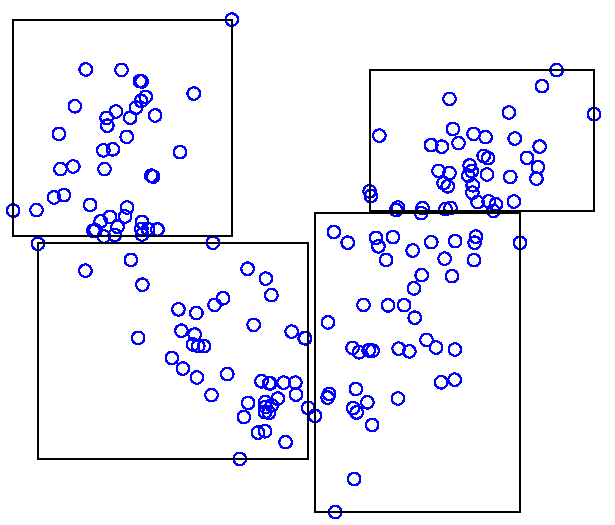
\includegraphics[width=0.45\textwidth]{images/kdtree-3}}
\subfigure[Last
level]{\label{fig:kdtree-4}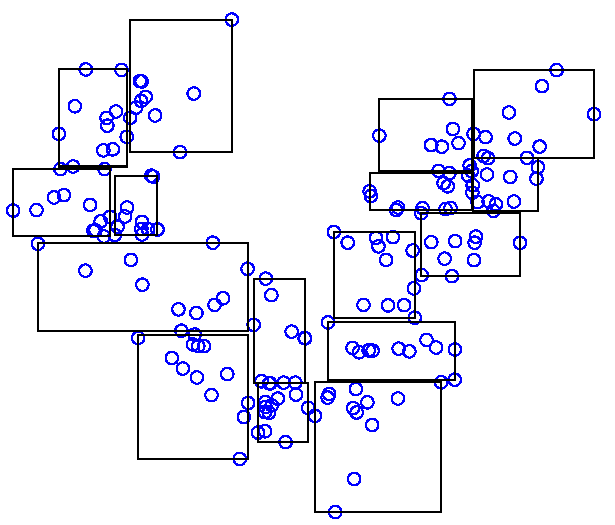
\includegraphics[width=0.45\textwidth]{images/kdtree-4}}
  \caption[$k$-d tree illustration]{Illustration of the $k$-d tree with bounding boxes at different
levels of depths. This figure also outlines the building phases of the tree.}
  \label{fig:kdtree}
\end{figure}

We start building the tree from the root node and then proceed in a recursive manner. At each
node we select which of the points from the current node will be allocated to each of
the two children. Because these are also described by hyper-rectangles, we just have to select a splitting plane. Then the two successors will consist of the points from the two sides of the hyper-plane. 

A splitting hyper-plane can be fully defined by two parameters: a direction $\vec{d}$ on which the plane is perpendicular and a point $P$  that is in the plane. Given that the splits are axis aligned, there are $D$ possible directions $\vec{d}$. We can either choose this randomly or we can use
each of the directions from $1$ to $D$ in a successive manner. A more common approach is to choose $\vec{d}$ to be the dimension that presents the largest
variance: 
\begin{align}
	\vec{d} \leftarrow \operatorname{argmax}_{d} (\max_ix_{id} -
\min_ix_{id}).
	\label{eq:splitting-direction}
\end{align}

Splitting perpendicular on the direction with the greatest variance results in a better clustering of the points and the shape of the bounding boxes will be closer to the shape of a square. Otherwise it might happen that points situated in the same node can still be further away.

Regarding the splitting value $P$, a usual choice is the median value $\tilde{x}_d$ on the previously selected direction $\vec{d}$. This choice of $P$ guarantees a balanced tree which offers several advantages. We can allocate static memory for the entire data structure. This is faster to access than dynamical allocation. Also a balanced tree has a better worst case complexity than an unbalanced one. Other useful implementation tricks that can be applied to balanced $k$-d trees are suggested by \cite{lang2009}.

After the splitting plane is chosen, the left child will contain the points that are on the left of the hyper-plane: 
\begin{align}
\mathcal{D}_{\le \tilde{x}_d} = \{ \xB \in \mathcal{D}_{\xB_i}| x_{d} \le \tilde{x}_d \},
\label{eq:subset-left}
\end{align}
 where $\mathcal{D}_{\xB_i}$ denotes the data points bounded by the current node $\xB_i$. Similarly, the right child will contain the points that are placed on the right of the hyper-plane:
\begin{align}
\mathcal{D}_{> \tilde{x}_d} = \{ \xB \in \mathcal{D}_{\xB_i}| x_{d} > \tilde{x}_d \}.
\label{eq:subset-right}
\end{align}

This process is repeated until the number of points bounded by the current node goes below a threshold $m$. These nodes are the leaves of the tree and they store the data points. The other non-leaf nodes store information regarding the bounding box and the splitting plane. A hyper-rectangle is completely defined by only two $D$-dimensional points, one for the ``top-right'' corner and the other for the ``bottom-left'' corner. 

	\begin{algorithm} 
		\caption{$k$-d tree building algorithm} 
		\label{alg:kd-tree-build}  
		\begin{algorithmic}[1]                    % enter the algorithmic environment
			\REQUIRE Data set $\mathcal{D}=\{\xB_1,\cdots,\xB_N\}$, $i$ position in tree
and $m$ number of points in leaves.
			\IF {$N < m$}
				\STATE Mark node $i$ as leaf: \texttt{splitting\_direction(i)=-1}.
				\STATE Add points to leaf: \texttt{points(i)}$\leftarrow \mathcal{D}$.
				\RETURN
			\ENDIF
				\STATE {Choose direction $\vec{d}$ using equation
\eqref{eq:splitting-direction}: \texttt{splitting\_direction(i)=}$d$.}
% 				\STATE {}
				\STATE {Find the median value $\tilde{x}_d$ on the direction $\vec{d}$: \texttt{splitting\_value(i)=}$\tilde{x}_d$.}
				\STATE {Determine the subsets of points that are separated by the resulting splitting plane: $\mathcal{D}_{\le\tilde{\xB}}$ and $\mathcal{D}_{>\tilde{\xB}}$, see equations \eqref{eq:subset-left} and \eqref{eq:subset-right}.}
				\STATE {Build left child
\texttt{build\_kdtree(}$\mathcal{D}_{\le\tilde{\xB}}$\texttt{,2*i)}.}
				\STATE {Build right child
\texttt{build\_kdtree(}$\mathcal{D}_{>\tilde{\xB}}$\texttt{,2*i+1)}.}
%							$\mathcal{D}_{>\tilde{\xB}}=\{\xB\in\mathcal{D}|\xB>\tilde{\xB}\}$
		\end{algorithmic}
	\end{algorithm}
	
 	The most common operation on a $k$-d tree is the nearest neighbour (NN) search. While we will not apply pure NN for the next method, we will use similar concepts. However, we can do NN retrieval with $k$-d trees after we applied NCA, as suggested by \citet{goldberger2004}. The search in the $k$-d tree is done in a depth-first search manner: start from the root and traverse the whole tree by selecting the closest node to the query point. In the leaf, we find the nearest neighbour from the $m$ points and store it and the corresponding distance $d_\text{min}$. Then we recurse up the tree and look at the farther node. If this is situated at a minimum distance that is smaller than $d_\text{min}$, we have to investigate also that node. Otherwise, we can ignore the node and all the points it contains. Usually, a large fraction of the points can be omitted, especially when the data is clustered.
 	It is important to stress that the performance of $k$-d trees quickly degrades with the dimensionality of the data. 
 	
 	%Hence, it is useful to understand how the search is done and how computational saving are achieved. 
	
%	\begin{itemize}
%		\item 
%		\item So we will be able to efficiently use $k$-d trees only when learning a
%low-rank $\AB$ that projects the data points in a low dimensional space.
%	\end{itemize}
	
%organize the data in a binary tree structure using axis-aligned splitting
%planes of the data space. Each node in the tree represents a data point and it
%also contains a splitting direction (this is usually denoted by an integer from
%1 to $k$). The splitting plane is often chosen to be perpendicular on the
%dimension with the largest variance and to go through the median point (this
%results in a balanced tree). Furthermore, a non-leaf node has two successors:
%the sub-tree rooted at the left successor contains the points that are situated
%at the left of the splitting plane, while the sub-tree rooted at the right
%successor of the splitting plane contains the points that are situated at the
%right of the splitting plane. 

\subsection{Approximate kernel density estimation}
\label{subsec:approx-kde}

The following ideas are mostly inspired by previous work on fast kernel density estimators with $k$-d trees \citep{gray2001, gray2003, gray2003b} and fast Gaussian Processes regression with $k$-d trees \citep{shen2006}.

In kernel density estimation (KDE), we are given a data set~$\mathcal{D}$ and the goal is to compute the probability denisty at a given point using a sum of the contributions from all the points:
\begin{align}
p(\xB_i) = \frac{1}{N}\sum_{j=1}^Nk(\xB_i|\xB_j).
\end{align}

A common class of KDE problems are the $N$-body problems \citep{gray2001} where we have to estimate $p(\xB_i)$ for each data point $\{\xB_i\}_{i=1}^N$ in the data set $\mathcal{D}$. This operation is quadratic in the number of points, as it is the case of NCA\@.

If the number of samples $N$ in $\mathcal{D}$ is sufficiently large, we
expect to accurately approximate $p(\xB_i)$ by using only nearby neighbours of $\xB_i$. 

To illustrate how this works, let us assume we are given a query point $\xB_i$ and a group of points $G$. We try to reduce computations by replacing each individual contribution $k(\xB_i|\xB_j), \xB_j\in G$, with a fixed quantity $k(\xB_i|\xB_g)$. The value of $k(\xB_i|\xB_g)$ is group specific and since it is used for all points in $G$, it is chosen such that it does not introduce a large error. 
A reasonable value for $k(\xB_i|\xB_g)$ is obtained by
approximating each point $\xB_i$ with a fixed $\xB_g$, for example, the mean of the points in $G$. Then we compute the kernel value $k(\xB_i|\xB_g)$ using the estimated $\xB_g$. A second possibility is to directly approximate $k(\xB_i|\xB_g)$. For example:
\begin{align}
  k(\xB_i|\xB_g) = \frac{1}{2}\left( k_{\min} + k_{\max} \right),
  \label{eq:approx-rule}
%\min_jk(\xB_i|\xB_j) + \max_jk(\xB_i|\xB_j)\right).
\end{align} 
where $k_{\min}$ and $k_{\max}$ represent the minimum and maximum contributions that can arise for the given query point~$\xB_i$ and the bounding box that encloses the group~$G$. This last option does not introduce any further computational expense. Both the minimum and the maximum contributions are previously calculated to decide whether to prune or not. Also it does not need storing any additional statistic, such as the mean.

The error introduced by each approximation is bounded by the following quantity:
\begin{align}
\epsilon_{\max} = \frac{1}{2}\left(k_{\max} - k_{\min}\right). 
\end{align}

This can be controlled to be small if we approximate only for those groups that are far away from the query point or when the variation of the kernel value is small within the group.
It is better still to consider the error relative to the total quantity~$p(\xB_i)$. Of course we do not know the total sum we want to estimate in advance, but we can use a lower bound: $p_{\text{SoFar}}(\xB_i) + N_Gk_{\min}$, where $p_{\text{SoFar}}$ denotes the current estimate for $p(\xB_i)$ and $N_G$ is the number of points in the group $G$. Hence, a possible cut-off rule is: 
\begin{align}
  \epsilon_{\max}N_G \le \tau (p_{\text{SoFar}} + N_Gk_{\min}),
\end{align}
where $\tau$ is a constant that controls the error introduced by the approximations: a small $\tau$ means the computations will more accurate, conversely, a large $\tau$ allows more approximations. We use a pruning technique whenever the cut-off rule is true. So in this case it is important the order in which we accumulate. A large $p_{\text{SoFar}}(\xB_i)$ in the early stages will allow more computational savings.

We use $k$-d trees to form groups of points $G$ that will be described as hyper-rectangles. To compute the probability density function $p(\xB_i)$, we start at the root, the largest group, and traverse the tree going through the nearest node each time until we reach the leaf. In this manner, we are able to add large contributions at the beginning. Then we recurse up the tree and visit other nodes only if necessary, when the cut-off condition is not satisfied. We give the exact algorithm for this procedure in the next subsection.

\subsection{Approximate KDE for NCA}
\label{subsec:approx-KDE-for-NCA}
 
We recall that NCA was formulated as a class-conditional kernel density estimation problem (CC-KDE; section \ref{sec:cc-kde}). By combining ideas from the previous two subsections, we can develop an NCA specific approximation algorithm.

There are some differences from the classical KDE approximation. In this case, we deal with class-conditional probabilities $p(\AB\xB_i|c),\forall c$. So each class $c$ needs to be treated separately: we build a $k$-d tree with the projected data points $\{\AB\xB_j\}_{j\in c}$ and calculate the estimated probability $\hat{p}(\AB\xB_i|c)$ for each class. Another distinction is that for NCA our final interests are the objective function and its gradient. Algorithm \ref{alg:cc-kde-nca} presents at a high-level how the NCA objective function and its gradient are computed in the CC-KDE scenario.

	\begin{algorithm}
		\caption{Approximate NCA} 
		\label{alg:cc-kde-nca}  
		\begin{algorithmic}[1]                    % enter the algorithmic environment
			\REQUIRE Projection matrix $\AB$, data set
$\mathcal{D}=\{\xB_1,\cdots,\xB_N\}$ and error~$\tau$.
			\FORALL {classes $c$}
				\STATE {Build $k$-d tree for the points in class $c$.}
			\ENDFOR 
			\FORALL {data points $\xB_i$}
				\FORALL {classes $c$}
					\STATE {Compute approximate class-conditional probability $\hat{p}(\AB\xB_i|c)$ and its
corresponding gradient $\frac{\partial}{\partial \AB} \hat{p}(\AB\xB_i|c)$ 
using algorithm \ref{alg:approx-cc-kde}}
%					\STATE {\texttt{[p(c),dp(c)]=NCA\_recursive(kdtree(c))}}
				\ENDFOR
				\STATE Compute soft probability $\hat{p}_i \equiv \hat{p}(c|\AB\xB_i) =
\frac{\hat{p}(\AB\xB_i|c_i)}{\sum_{c}\hat{p}(\AB\xB_i|c)}$.
				\STATE Update function value (equation \ref{eq:nca-cc-kde-obj}) and gradient value
				(equation \ref{eq:nca-cc-kde-grad}).
			\ENDFOR
		\end{algorithmic}
	\end{algorithm}

We demonstrate how we can obtain an approximated version of the objective function. We begin by replacing $p(\AB\xB_i|c)$ with the approximated $\hat{p}(\AB\xB_i|c)$ in equation~\eqref{eq:nca-cc-kde-obj}:
\begin{align}
	    \hat{f}(\AB) = \sum_{i=1}^{N} \hat{p}(c_i|\AB\xB_i).
	    \label{eq:nca-cc-kde-obj-approx}
\end{align}

To obtain the gradient of this new objective function we use equation~\eqref{eq:nca-cc-kde-grad}. We remind that each individual contribution is given by a normal distribution:
\begin{align}
  k(\AB\xB|\AB\xB_i) \propto \exp\left\{ -(\AB\xB - \AB\xB_i)\tr(\AB\xB - \AB\xB_i) \right\}.
\end{align}

So the gradient of each individual contribution with respect to the linear transformation~$\AB$ will be:
\begin{align}
  \frac{\partial}{\partial \AB} k(\AB\xB|\AB\xB_i) \propto -2\AB\cdot k(\AB\xB|\AB\xB_i)(\xB-\xB_i)(\xB-\xB_i)\tr.
\end{align}

Now let us consider the derivative~$\frac{\partial}{\partial \AB}{p}(\AB\xB|c)$ for a group $G$ and  then approximate it using the criterion given in equation~\eqref{eq:approx-rule}. We obtain:
		\begin{align}
		  \frac{\partial}{\partial \AB} p(\AB\xB|G)&=\frac{\partial}{\partial \AB} \sum_{j\in G} k(\AB\xB|\AB\xB_j)\notag\\
			&\approx\frac{\partial}{\partial \AB} \frac{1}{2} \left( k_{\min} + k_{\max} \right)\notag\\
			& = \frac{1}{2}\left\{ \frac{\partial}{\partial \AB} k(\AB\xB|\AB\xB_c) +
\frac{\partial}{\partial \AB} k(\AB\xB|\AB\xB_f) \right\}\notag\\
			& = -\AB\left\{ k_{\max}(\xB-\xB_c)(\xB-\xB_c)\tr +
			k_{\min}(\xB-\xB_f)(\xB-\xB_f)\tr \right\},
		\label{eq:nca-kde-approx-pAXc}
	\end{align}
		where $\AB\xB_c$ and $\AB\xB_f$ denote the points associated to $k_{\max}$ and~$k_{\min}$. % We can determine $k_{\min}$ and $k_{\max}$ by making use of the fact the kernel function is a monotonic function of the distance: the closest point gives the maximum contribution, while the farthest point the minimum. The  minimum distance
		We observe that for the gradient computation we need to find these points and then to recover their positions in the original space. The class-conditional approximated gradient is obtained by adding the contributions for all the groups (algorithm~\ref{alg:approx-cc-kde}).
		%give the closest point in $G$ to the query point $\AB\xB$ and $\AB\xB_f$ is the farthest point in $G$ to $\AB\xB$. 
		%Here we made use of the fact the kernel function is a monotonic function of the distance. This means that the closest point gives the maximum contribution, while the farthest point the minimum.
		%We see that equation~\eqref{eq:nca-kde-approx-pAXc} cannot be applied for estimating the gradient of the objective function. The gradient depends on the positions of the points in original space and neither $\AB\xB_c$ nor $\AB\xB_f$ belong to our data set so we cannot recover the positions. Both the minimum and the maximum contribution have associated a point in the bounding box. But since the bounding box is formed in the low dimensional space using $\{\AB\xB_i\}_{i=1}^N$ we cannot the points 

	\begin{algorithm}
		\caption{Approximate class-conditional kernel density estimation} 
		\label{alg:approx-cc-kde}  
		\begin{algorithmic}[1]                    % enter the algorithmic environment
			\REQUIRE Query point $\xB$, projection matrix $\AB$, data set
$\mathcal{D}=\{\xB_1,\cdots,\xB_N\}$ and error~$\tau$.
			\STATE Find $d_{\max}$ and $d_{\min}$ from $\xB$ to the current bounding box and then compute $k_{\min}$ and $k_{\max}$.
			\IF {$N_G(k_{\max}-k_{\min}) \le 2\tau (p_{\text{SoFar}} + N_Gk_{\min})$}
				\STATE Compute group contribution: {$\hat{p}(\AB\xB|G) = \frac{N_G}{2}\left( k_{\min} + k_{\max} \right)$}
				\STATE Compute derivative~$\frac{\partial}{\partial\AB}\hat{p}(\AB\xB|G)$ using equation~\eqref{eq:nca-kde-approx-pAXc}
				\STATE Update accumulated contribution: $p_{\text{SoFar}}\leftarrow p_{\text{SoFar}}+\hat{p}(\AB\xB|G)$
				\RETURN  $\hat{p}(\AB\xB|G)$ and $\frac{\partial}{\partial\AB}\hat{p}(\AB\xB|G)$.
			\ENDIF
			\IF {current node is a leaf}
				\STATE {Compute probability: $p(\AB\xB|G_\text{leaf})=\sum_{j\in\text{leaf}}k(\AB\xB|\AB\xB_j)$}
				\STATE {Compute derivative: $\frac{\partial}{\partial \AB} p(\AB\xB|G_\text{leaf})=\frac{\partial}{\partial \AB} \sum_{j\in G_\text{leaf}} k(\AB\xB|\AB\xB_j)$}
				\STATE {Update $p_\text{SoFar}$}
				\RETURN  $p(\AB\xB|G_\text{leaf})$ and $\frac{\partial}{\partial\AB}p(\AB\xB|G_\text{leaf})$.
			\ENDIF
			\STATE {Recurse on nearest child to $\xB$ and compute the probability and the gradient contributions: 
					$\hat{p}(\AB\xB|G_{\text{near}})$ and $\frac{\partial}{\partial\AB}\hat{p}(\AB\xB|G_{\text{near}})$}
			\STATE {Recurse on farthest child to $\xB$ and compute the probability and the gradient contributions: 
					$\hat{p}(\AB\xB|G_{\text{far}})$ and $\frac{\partial}{\partial\AB}\hat{p}(\AB\xB|G_{\text{far}})$}
			\RETURN $\hat{p}(\AB\xB|G_{\text{near}}) + \hat{p}(\AB\xB|G_{\text{far}})$ and $\frac{\partial}{\partial\AB}\hat{p}(\AB\xB|G_{\text{near}})+\frac{\partial}{\partial\AB}\hat{p}(\AB\xB|G_{\text{far}})$.
		\end{algorithmic}
	\end{algorithm}
	
	
\section{Exact computations}
\label{sec:exact-computations}

	Exact methods are the counterpart of approximate methods. We can have both efficient and exact computations just by modifying the NCA model. Again, the idea is motivated by the rapid decay of the
	exponential function. Instead of operating on very small values, we will make them exactly zero. This is achieved by replacing the squared exponential kernel with a compact support function. So, the points that lie outside the support of the kernel are ignored and just a fraction of the total number of points is used for computing the contributions~$p_{ij}$. The most significant cost savings come from the fact we do not have to compute the expensive gradient terms for the points that have $p_{ij}=0$. Further gains in speed are obtained if the search for those points is done with $k$-d trees (the range search algorithm is suitable for this task; \citealp{moore1991}).
	
	The choice of the compact support kernel is restricted by a single requirement: differentiability. We will use the simplest polynomial function that has this property. This is given by the
	following expression:
	\begin{align}
		k_{\text{CS}}(u)=\begin{cases}
			h(a^2-u^2)^2& \mbox{if } u \in [-a;+a]\\
			0& \mbox{otherwise},\\
		\end{cases}
		\label{eq:cs-1}
	\end{align}
	where $h$ is a constant that controls the height of the kernel and $a$ is a constant that controls the width of the kernel. In the given context, the kernel will be a function of the distance between two points: $k_{\text{CS}}(u)=k_{\text{CS}}(d_{ij})$, where $d_{ij} = d(\AB\xB_i;\AB\xB_j)$. 
	
	We introduced a general expression for the compact support kernel because later we will need to carefully set the parameters $a$ and $h$ (subsection~\ref{sec:nca-cs-back}). For now, we can consider $a=1$ and $c=1$. We obtain the following simplified version of the kernel:
%	Note that the constant $a$ can be absorbed by the linear projection $\AB$. This means that the scale of the learnt metric will compensate for the kernel's width. Also the value for $c$ is not important: from equation \eqref{eq:stochastic-neighbours-cs} we see that this reduces. 
	\begin{align}
		k_{\text{CS}}(d_{ij})= (1-d_{ij}^2)^2\;\mathrm{I}(\left|d_{ij}\right|\le1),
	\end{align}
	where $\mathrm{I}(\cdot)$ denotes the indicator function: $\mathrm{I}(\cdot)$ return 1 when its argument is
	true and 0 when its argument is false.
	
	Now we reiterate the steps of the NCA algorithm (presented in section \ref{sec:general-presentation}), and replace $\exp(\cdot)$ with $k_\text{CS}(\cdot)$. We obtain the following new stochastic neighbour assignments:
	\begin{align}
		q_{ij} = \frac{k_{\text{CS}}(d_{ij})}{\sum_{k\neq i} k_{\text{CS}}(d_{ik})}.
		\label{eq:stochastic-neighbours-cs}
	\end{align}
	
	These can be compared to the classical soft assignments given by equation~\eqref{eq:stochastic-neighbour}. Next we do not need to change the general form of the objective function: 
	\begin{align}
		f_\text{CS}(\AB) = \sum_{i}\sum_{j\in c_i} q_{ij}.
	\end{align}
	
	In order to derive the gradient of the function $f_\text{CS}$, we start by computing the gradient of the kernel:
	\begin{align}
		\frac{\partial}{\partial\AB}k_\text{CS}(d_{ij}) 
		&= 
	\frac{\partial}{\partial\AB}\left[(1-d_{ij}^2)^2\cdot\mathrm{I}(\left|d_{ij}\right|\le
	1)\right]\notag\\
		&= -4\AB(1-d_{ij}^2)  \xB_{ij} \xB_{ij}^\mathrm{T} \cdot
	\mathrm{I}(\left|d_{ij}\right|\le 1),\label{eq:nca-cs-grad-kernel}
	\end{align}
	where $\xB_{ij}=\xB_i-\xB_j$.
	
	The gradient of the new objective function is:
	\begin{align}
		\frac{\partial f_\text{CS}}{\partial \AB}=4\AB\sum_{i=1}^{N}
		\left(
		q_i \sum_{k=1}^N \frac{q_{ik}}{1-d_{ik}^2} \xB_{ik}\xB_{ik}^{\textrm{T}}
		- \sum_{j\in c_i} \frac{q_{ij}}{1-d_{ij}^2}\xB_{ij}\xB_{ij}^{\textrm{T}} 
		\right).
		\label{eq:nca-cs-grad}
	\end{align}
	
	This method can be applied in same way as classic NCA: learn a metric $\AB$ that maximizes the objective function $f_\text{CS}(\AB)$. Since the function is differentiable, any gradient based method is suitable for optimization and can be used on equation~\eqref{eq:nca-cs-grad}.
	
	There is one concern with the compact support version of NCA. There are situations when a point $\xB_i$ is placed outside the support of any other point in the data set. Intuitively, this means that the point $\xB_i$ is not selected by any point, hence it is not assigned any class label. Also this causes mathematical problems: as in subsection \ref{subsec:numerical-issues}, the contributions $p_{ij}$ will have an indeterminate value $\frac{0}{0}$. The advice from subsection \ref{subsec:numerical-issues} can be applied here as well. A more robust way of dealing with this is discussed in the next subsection.
	
%	The main concern with this method is what happens when points lie outside the
%	compact support of any other point in the data set. So care must be taken at
%	initialisation. One way would be to initialise with a very small scale $\AB$.
%	However, this means that there is no gain in speed for at least the first
%	iterations. It might be better to use the principal components for
%	initialisation. 
	
\subsection{NCA with compact support kernels and background distribution}
\label{sec:nca-cs-back}

	\begin{figure}
	  \centering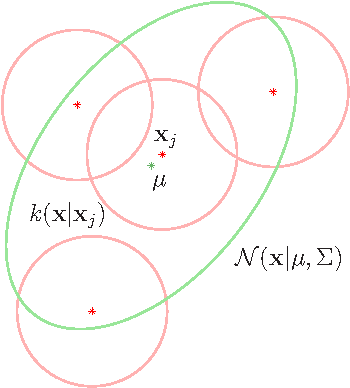
\includegraphics[width=6cm]{images/nca-cs-back}
	  \caption[NCA with compact support kernels and normal background distribution]{Neighbourhood component analysis with compact support kernels and
	background distribution. The main assumption is that each class is a mixture of
	compact support distributions $k(\xB|\xB_j)$ plus a normal background
	distribution $\mathcal{N}(\xB|\muB,\SigmaB)$.}
	  \label{fig:cs-back}
	\end{figure}
	
	We extend the previous model to handle cases where points fall outside the support of any other neighbours. The idea is to use  for each class a background distribution that explains the unallocated points. The background distribution should have an infinite support and an obvious example is the normal distribution.
	
	To introduce a background distribution in a principled manner, we return to the class conditional kernel density estimation (CC-KDE) formulation of NCA (section \ref{sec:cc-kde}). First, we recast the compact support NCA in the probabilistic framework and consider each class as mixture of compact support distributions: 
	\begin{align}
		p(\xB_i|c) = \frac{1}{N}\sum_{j\in c} k_\text{CS}(\xB_i|\xB_j),
	\end{align}
	where $k_\text{CS}(\xB_i|\xB_j) = k_\text{CS}(d_{ij})$ and is defined by equation~\eqref{eq:cs-1}. Because $k_\text{CS}(\xB_i|\xB_j)$ denotes a distribution, it ought to integrate to 1. For $h=\frac{15}{16}$ and $a=1$ the requirement is satisfied.
	
	We further change the model and incorporate an additional distribution in the class-conditional probability $p(\xB_i|c)$. From a generative perspective this can be interpreted as follows: a point $\xB_i$ is generated by either the compact support distribution from each point $k_\text{CS}(\xB_i|\xB_j)$ or by a class-specific normal distribution $\mathcal{N}(\xB_i|\muB_c,\SigmaB_c)$. So, the distribution $p(\xB_i|c)$ can be written as the sum of these components:
		\begin{align}
			p(\xB_i|c) = \beta \mathcal{N}(\xB_i|\muB_c,\SigmaB_c) + (1-\beta)
	\frac{1}{N_c}\sum_{j\in c} k_\text{CS}(\xB_i|\xB_j),
			\label{eq:nca-cs-back-1}
		\end{align}
	where $\beta\in[0,1]$ is the mixing coefficient between the background distribution and
	the compact support model, $\muB_c$ is the sample mean of the class $c$ and $\SigmaB_c$ is the sample
	covariance of the class $c$. The constant $\beta$ can be set to $\frac{1}{N_c+1}$. This will give equal weights to the background distribution and to each compact support distribution. It might be better to treat $\beta$ as a parameter and fit it during training. We expect $\beta$ to adapt to the data set: for example, $\beta$ should increase for data sets with convex classes. 
	
	To finalize this method, we just need to plug equation \eqref{eq:nca-cs-back-1} into
	the set of equations \eqref{eq:nca-cc-kde-bayes}, \eqref{eq:nca-cc-kde-obj} and
	\eqref{eq:nca-cc-kde-grad}. The only difficulty is the gradient computation. We now give the derivatives for each individual component:
	\begin{itemize}
%		\item $\beta = \frac{1}{N_c+1}$ we will give equal weights to the background
%	distribution as to the compact-support distribution. Setting it too large means
%	that the model will favour convex classes. On one hand, this might diminish
%	NCA's power. One of its strengths lies in the ability to work on non-convex
%	classes. On the other hand, some of the classes  This can be fitted as a
%	parameter during the optimization process. The gradient with respect to $\beta$
%	can be easily derived and it is easy to evaluate it as the quantities required
%	for this should also be computed for the function evaluation. 
		\item The gradient of the compact support distribution $k_\text{CS}(\xB_i|\xB_j)$ with respect to $\AB$ is very similar to what is given in equation \eqref{eq:nca-cs-grad-kernel}. The only difference is that in this case we have everything multiplied by the constant $h=\frac{15}{16}$.
		\item For the gradient of the background distribution it is useful to note that projecting the points $\{\xB_i\}_{i=1}^N$
	into a new space $\{\AB\xB_i\}_{i=1}^N$ will change the sample mean $\muB_c$ to
	$\AB\muB_c$ and the sample covariance $\SigmaB_c$ to
	$\AB\SigmaB_c\AB^\mathrm{T}$. Hence, we have:
		\begin{align}
			\frac{\partial}{\partial \AB} \mathcal{N}(\AB\xB_i&|\AB\muB_c, \AB\SigmaB_c
	\AB^\mathrm{T}) = \mathcal{N}(\AB\xB_i|\AB\muB_c, \AB\SigmaB_c
	\AB^\mathrm{T})\notag\\
			&\times \{ -(\AB\SigmaB_c \AB^\mathrm{T})^{-1}\AB\SigmaB_c
			+\vB \vB ^ \mathrm{T} \AB \SigmaB_c - \vB (\xB - \muB_c)^\mathrm{T}
			\},
		\end{align}
		where $\vB = (\AB\SigmaB_c \AB^\mathrm{T})^{-1}\AB(\xB - \muB_c)$.
		\item If we also consider $\beta$ a parameter, we also need the derivative of the objective function with respect to $\beta$. This can be easily obtained, if we use the derivative of the class conditional distribution with respect to $\beta$:
		\begin{align}
			\frac{\partial}{\partial\beta} p(\xB_i|c) 
			=  \mathcal{N}(\xB_i|\muB_c,\SigmaB_c) -
				\frac{1}{N_c}\sum_{j\in c} k_\text{CS}(\xB_i|\xB_j).
		\end{align}
	\end{itemize}
	
	We obtain a suitable the metric~$\AB$ in the standard way, by using a gradient-based optimizer.
	
	\section*{Summary}
	\label{sec:summary}
	
	In this chapter we have shown two main families of algorithms that can help reducing the computational cost of NCA\@. First, we have considered mini-batch algorithms. These achieve speed-ups by using sub-sets of the data instead of the whole training set. Second, we have presented algorithms that are based on approximations. In section~\ref{sec:approximate} we saw how the NCA function can be directly approximated using $k$-d trees, while in section~\ref{sec:exact-computations} we propose a different model to get the same effect even if we did not introduce approximation errors. Finally, in subsection~\ref{sec:nca-cs-back} we make the compact support classifier well defined across the whole space by using a Gaussian distribution to represent each class. The next chapter will present the results obtained by evaluating these methods and a comparison between different algorithms.